% use paper, or submit
% use 11 pt (preferred), 12 pt, or 10 pt only

\documentclass[letterpaper, preprint, paper,11pt]{AAS}	% for preprint proceedings
%\documentclass[letterpaper, paper,11pt]{AAS}		% for final proceedings (20-page limit)
%\documentclass[letterpaper, paper,12pt]{AAS}		% for final proceedings (20-page limit)
%\documentclass[letterpaper, paper,10pt]{AAS}		% for final proceedings (20-page limit)
%\documentclass[letterpaper, submit]{AAS}			% to submit to JAS
\usepackage{bm}
\usepackage{amsmath}
\usepackage{subfigure}
%\usepackage[notref,notcite]{showkeys}  % use this to temporarily show labels
\usepackage[colorlinks=true, pdfstartview=FitV, linkcolor=black, citecolor= black, urlcolor= black]{hyperref}
\usepackage{overcite}
\usepackage{footnpag}			      	% make footnote symbols restart on each page
\usepackage{listings}                   % Code Listings
\usepackage{xcolor}                     % Code Coloring
\usepackage[explicit]{titlesec}         % Paragraph Headers
\usepackage{ulem}                       % Paragraph Headers Underlines

% CREATING PARAGRAPH HEADERS
\titleformat{name=\paragraph,numberless}[runin]
    {\normalfont\normalsize\bfseries}{}{15pt}{\uline{#1}}

% DEFINING CODE COLORS
\definecolor{comments}{rgb}{0.0, 0.5, 0.0}
\definecolor{keywords}{rgb}{0.01, 0.28, 1}

\lstset{
    basicstyle = \small\ttfamily,
    language = Python,
    frame = lines,
    backgroundcolor = \color{lightgray!10},
    commentstyle = \color{comments}\ttfamily\small,
    keywordstyle = \color{keywords}\bf\ttfamily\small,
    framesep=\fboxsep,
}
% \lstset{
%     % language={[LaTeX]TeX},
%     %alsolanguage={PGF/TikZ},
%     frame=single,
%     framesep=\fboxsep,
%     framerule=\fboxrule,
%     % rulecolor=\color{red},
%     xleftmargin=\dimexpr\fboxsep+\fboxrule,
%     xrightmargin=\dimexpr\fboxsep+\fboxrule,
%     breaklines=true,
%     basicstyle=\small\tt,
%     keywordstyle=\color{blue}\sf,
%     % identifierstyle=\color{magenta},
%     % commentstyle=\color{cyan},
%     % backgroundcolor=\color{yellow!10},
%     tabsize=2,
%     columns=flexible,
% }


\PaperNumber{20-686}



\begin{document}

\title{IMPLEMENTATION OF DEEP SPACE MANEUVERS IN BROAD SEARCH TRAJECTORIES USING MONTE CARLO TREE SEARCH}

\author{Burton A. Yale\thanks{Undergraduate Student, Aerospace Engineering, Cal Poly Pomona, 3801 W Temple Ave, E-mail: bayale@cpp.edu},  
Jehosafat J. Cabrera\thanks{Undergraduate Student, Aerospace Engineering, Cal Poly Pomona, 3801 W Temple Ave, E-mail: jehosafatc@cpp.edu},
\ Rohan D. Patel\thanks{Undergraduate Student, Aerospace Engineering, Cal Poly Pomona, 3801 W Temple Ave, E-mail: rohanpatel@cpp.edu},
\ and Navid Nakhjiri\thanks{Assistant Professor, Aerospace Engineering, Cal Poly Pomona, 3801 W Temple Ave, E-mail: nnakhjiri@cpp.edu}
}


\maketitle{} 		


\begin{abstract}
Multiple flybys of the inner planets and the application of $V_{\infty}$ leveraging are essential trajectory design techniques to reduce the required launch energy for interplanetary missions. These trajectories are often difficult to formulate and require extensive computational resources. However, this problem can be classified as a sequential planning task which can be solved by a Monte Carlo Tree Search (MCTS) method. In this paper, a MCTS algorithm is developed and tested with a focus on reducing required $\Delta$V from the spacecraft. This method balances exploration and exploitation of the search space, and the algorithm’s performance is assessed by tweaking the selection policy parameter. Optimizations of several cases are studied to prove the feasibility of the tree search results. The algorithm will allow for inner-planetary flyby search planning for outer planetary missions.
\end{abstract}

\section{Introduction}
Broad trajectory searches are one fo the first steps in mission planning, allowing for the selection of candidates given a list of constraints and a search space. As is the nature with combinatorial problems, every additional flyby adds another dimension to the search space. Brute force methods lead to expensive but thorough results. By pruning possible choices before the each selection, the overall computation time can be decreased, at the expense of losing possible results. There have been various approaches to this method, from evolutionary/genetic algorithms, to particle swarm optimization, to enumerated searches, all with their own benefits and drawbacks. The method of interest for this algorithm was enumerated searches, a subset of grid searches, as recent work has proven their ability to quickly and accurately find multi-leg interplanetary trajectories\cite{Hennes2015}.

\textbf{M}onte \textbf{C}arlo \textbf{T}ree \textbf{S}earch (MCTS), is a heuristics-based adaptation of the enumerated search, has the ability to both explore and exploit its environment. This allows the algorithm to find the narrow bands where multiple planet combinations are possible and exploit them to complete its goal. As such, larger search spaces can be employed without exponential growth in computation time.

This algorithm will deliver a set of planetary sequences and the dates associated that meet mission criteria, such as destination, launch windows, total fuel budgets, etc. These results can then be passed on to the next phase of the design, optimization 


\section{Background}

Interplanetary mission design is an iterative process. First, a sequence of encounter bodies is selected and is followed by evaluating all possible trajectories for that specified sequence. In literature, this is often referred to as pathfinding and path solving respectively [3]. In preliminary design, due to the increasing complexity of gravity assists and combinatorial solutions, a low-fidelity tool is generally utilized first to find regions of interest. This is then followed by a high-fidelity tool which searches through prospective and highly valued regions. These low-fidelity tools make use of algorithms to decrease computation time while increasing the number of possible solutions. 

Grid-search, for instance has been previously used as a search algorithm to find possible trajectories to KBOs [4]. Grid search is a type of search algorithm with the ability to map the entire search space so that there are no regions of interest missed. This method has been used to properly parametrize the time of flight between encounter bodies. In this manner, Earth having a period of 365 days will have the same number of possible encounters as Jupiter with a period of approximately 12 years [2]. Thus, the output grid will be that of an angular grid as opposed to a cartesian grid. This type of search algorithm, however, can be expensive in terms of computing power and time. To alleviate both of these constraints, heuristics can be implemented into the program. 

Beam Search (BS), a heuristic tree search algorithm, can be used as a searching criterion to find a sequence of planets from which gravity-assist from [4]. BS uses the method of Breadth-First Search (BFS) to search the tree of possibilities. BS builds each layer of the tree and orders the nodes in accordance to their heuristic cost. However, it only chooses those nodes with a maximum value to build from. Depth-First Search (DPS), alternatively, is used as a searching criterion to traverse down the tree [5]. Opposite to BFS, DPS does not search the tree at every level but rather explores a branch until the termination criteria is met. After which, moving in reverse updates the branch and moves towards the root node to start the process again. Both the BFS and DPS, search and prune the search-space consecutively. Using the Lazy Race Tree Search, the search space is pruned, and nodes ranked through the time of flight [5]. The use of heuristics avoids finding redundant solutions and increases the efficiency of the method used. Izzo et. al. [2] proposed the use of the Monte Carlo Tree Search to find fast solutions to interplanetary trajectories. 

The search sensitivity criteria of DPS, BS, and BFS are explored in conjunction with that of the MCTS and compared. These searches, however, did not take into account Deep Space Maneuvers (DSMs) and led to trivial solutions when trying to validate the Rosetta Trajectory. The validation and correct recreation of this mission will be the basis of the algorithm taking into account DSMs to fully model Leveraging Orbits.

\section{Monte Carlo Tree Search Implementation}

This tree is built upon a set of individual nodes, that are all connected to each other through their parent and children, much like a family tree. Each node has an associated state to represent a leg in the tour of a spacecraft, with a planetary body, and the time at which it is encountered. The process of building the tree throughout a run of the algorithm can be characterized by four essential steps: selection, expansion, simulation, and backpropagation. Figure~\ref*{fig:mctsFunc} depicts how the tree changes with respect to each phase of the MCTS loop. 
%At the start of each iteration, the program will begin at the root of the tree, and select down the tree until a leaf node is reached. From this leaf, the algorithm will expand a set of new child states and choose from the new selection. To generate an expected future reward from this node, the program will conduct a randomly stepped search until termination conditions are met. 
%After a fixed set of iterations of this process has been conducted, the algorithm will gather all leaf nodes, nodes with no children, that meet the user-defined criteria.

\begin{figure}[htb]
	\centering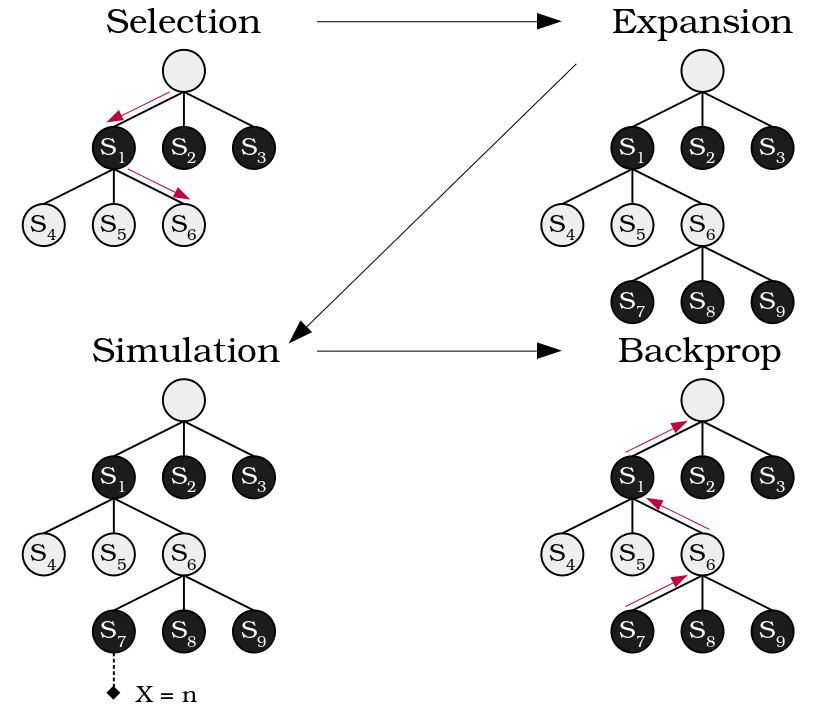
\includegraphics[width=3.5in]{fig/mctsFuncs.png}
	\caption{4 Main Steps for the Creation of a Monte Carlo Tree}
	\label{fig:mctsFunc}
\end{figure}

\subsection{Selection} 
At the start of each iteration, the program begins at the root of the tree $id = 0$, and from its children, select the child with the highest associated UCB1 value. With $X$ being the future reward from exploring the node, $N$ being the number of visits the node has recieved, and $n$ being the number of visits the parent node has recieved. 
\begin{equation*}
    \text{UCB1 Node Value: } X + C_p \sqrt{\frac{\ln{n}}{N}}
\end{equation*}

In the case of $C_p$, the exploration-exploitation parameter, a value of $C_p = \frac{1}{\sqrt{2}}$ was selected due to its performance in [Hennes and Izzo, 2015]. 

As the function selects down the tree, it evaluates the all children of each node for is they lead to a terminal condition, such as running out of the fuel budget. If all child nodes are considered terminal, then the associated parent node is also considered terminal, and the function restarts at the top of the tree. This process was implemented in order to prune the tree of any branches that showed results initially, but lead to all terminal states. Once the function has reached a leaf node, it will return the id associated and move onto the next step in building the tree, expansion.

\subsection{Expansion}
Before the creation of the new set of nodes, the function will first look at the state of the current node being expanded from as a base. As planetary motion is a problem involving conic sections, cartesian grid position sampling is not viable, thus angular divisions are required to efficiently sample a planets position. When selecting states for new nodes, the following policy is implemented. 
\begin{equation*}
    E = 
    \left(\begin{array}{c}
        n*(\tau_1 + \tau_0) + t_0 \\ 
        \vdots \\
        m*(\tau_1 + \tau_0) + t_0 \\
    \end{array}\right)
    \text{ for } 
    \left\{\begin{array}{llr} 
        n = 0.1, & m = 1.0 &\text{if } a_1 < 2 \text{ AU} \\ 
        n = 0.05, & m = 0.25 &\text{if } a_1 \geq 2 \text{ AU}
    \end{array}\right.
\end{equation*}

For the ephemeris time array $E$, the time of flight of the Lambert arc is dictated by the period of the planet state of the child node, $\tau_1$, and the period of the planet state of the parent node, $\tau_0$. This array is bounded using the parameters $n$ and $m$, which are defined by the semi-major axis of the child node's planet, $a_1$. The values for $n$ and $m$ were determined based on the performance of the tree, for outer planet destinations, early, faster, arrivals were prefered, so their parameters have been reduced to reflect as such. 

With the upper and lower bounds of the array set, an additional parameter, defined by the user, $d$ specifies the length of the array, also defining the resolution of the time steps. For the purpose of this paper, a value of $d = 16$ was found to be sufficient for all calculations as a balance between computation time and detail. 

Once the list of states has been established, a new set of children nodes are created to match all combinations of ephemeris times and planetary id pairs. In order to further prune the tree to reduce unnecessary calculations, Lambert arcs are calculated to each state pair to evauluate their associated $\Delta \text{v}$ cost. Any node that exceeds the mission budget is considered terminal and not used in any further exploration.

In order to calculate mission $\Delta \text{v}$ usage, the simulation uses powered flybys, as characterized by [Wei] \textbf{MORE HERE LATER}
\[ a_\text{in/out} = -\frac{\mu_p}{v^2_{\infty-\text{in/out}}} \]
\[ \delta = \text{cos}^{-1}\left(\frac{ \vec{\textbf{v}}_{\infty-\text{in}} \cdot \vec{\textbf{v}}_{\infty-\text{out}} }{ v_{\infty-\text{in}} \cdot v_{\infty-\text{out}} }\right) \]
\[ f =  \]
\[ \frac{\text{d}f}{\text{d}e_{out}} =  \]
\[ r_p = a_{in}(1 - e_{in}) = a_{out}(1 - e_{out}) \]
\[ \Delta V_{fb} = \left| \sqrt{v^2_{\infty-\text{in}} + \frac{2\mu_p}{r_p}} - \sqrt{v^2_{\infty-\text{out}} + \frac{2\mu_p}{r_p}} \right| \]

\subsection{Simulation}



\subsection{Backpropagation}

\section{Deep Space Maneuvers Implementation}

\begin{itemize}
    \item Rohan how dsm's work
    
    \item I talk about how its implemented
\end{itemize}

\section{Performance Evaluation}

\subsection{Leveraging Maneuver to Saturn}


\begin{itemize}
    \item Figures
        \item States (Seq vs Vinf)
    \item Tables
        \item MCTS Inputs
\end{itemize}

\subsection{Europa Clipper Trajectory Recreation}


\begin{itemize}
    \item Figures
        \item States (tof vs vinf)
        \item MALTO
    \item Tables
        \item MCTS Inputs
        \item MCTS Outputs
\end{itemize}

\subsection{Triton Trajectory Recreation}
Exploratory

\begin{itemize}
    \item Figures
        \item States 
        \item MCTS Trajectory Families
    \item Tables
        \item MCTS Inputs
\end{itemize}

\begin{lstlisting}
def mcts.run():
    for _ in maxIterations:
        if all(launchNodes is terminal):
            break

        # Select Most Valuable Leaf Starting from Root
        id = select() 

        # Expand If Prevously Visited and Pick Most Valuable Child
        if node.children is None and node.visits is not 0:
            id = expand(id)

        # Randomly Explores From Selected Node To Generate Cost
        X = simulate(id) 

        # Propagates Results Up Branch
        backprop(id, X)
\end{lstlisting}

\appendix
\bibliographystyle{AAS_publication}   % Number the references.
\bibliography{references}   % Use references.bib to resolve the labels.

\end{document}